\documentclass[]{usiinfprospectus}

\captionsetup{labelfont={bf}}

\author{\centerline{Bevilacqua Joey} \\[3pt] \centerline{De Vita Gianmarco}  \\[3pt] \centerline{Luini Alessandro}  \\[3pt] \centerline{Maggioni Claudio}}

\title{\centerline{Sudoku}}
\versiondate{\today}
\usepackage{boldline} 
\usepackage{enumitem}

\abstract {
The aim of this project is to make an Encoder and Decoder for a SAT-solver in order to decide whether a problem is satisfiable or unsatisfiable. WRITE A BETTER ABSTRACT
}

% For Sudoku drawing
\usepackage{tikz}
\newcounter{row}
\newcounter{col}

\newcommand\setrow[9]{
  \setcounter{col}{1}
  \foreach \n in {#1, #2, #3, #4, #5, #6, #7, #8, #9} {
    \edef\x{\value{col} - 0.5}
    \edef\y{9.5 - \value{row}}
    \node[anchor=center] at (\x, \y) {\n};
    \stepcounter{col}
  }
  \stepcounter{row}
}

\begin{document}
\maketitle
\tableofcontents
\newpage
%%%%%%%%%%%%%%%%%%%%%%%%%
\section{Introduction} \label{introduction}
\section{Problem definition} \label{problem}
Sudokus are puzzles based upon number placement. They are classically structured in a $9\times 9$ grid with 81 cells, divided into $3\times 3$ boxes. In order to be satisfiable, the following statements must hold:
\begin{itemize}%[label={(\arabic*)}]
\item In every cell there is exactly one number $c \in \{1, 2, ..., 9 \}$
\item No number may appear more than once in the same row or column.
\item No number may appear more than once in the same box.
\end{itemize}
Often Sudoku puzzles are initialized with some values placed.

%Draw Sudoku
\begin{figure}[h]
\begin{center}
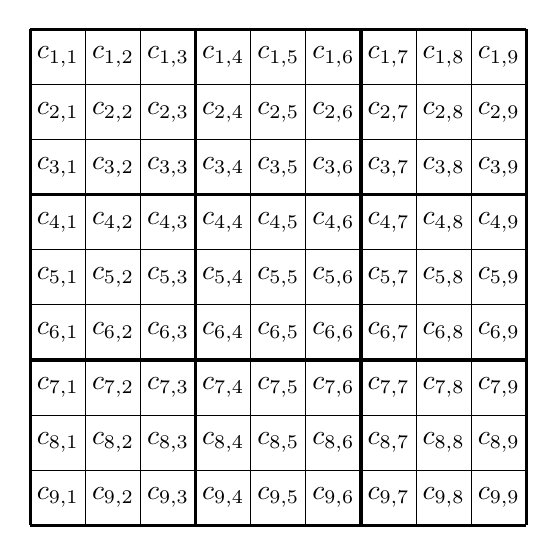
\begin{tikzpicture}[scale=.7]
  \begin{scope}
    \draw (0, 0) grid (9, 9);
    \draw[very thick, scale=3] (0, 0) grid (3, 3);

    \setcounter{row}{1}
    \foreach \i in {1,...,9}
    {
    \setrow {$c_{\i,1}$ }{$c_{\i,2}$}{$c_{\i,3}$}  {$c_{\i,4}$}{$c_{\i,5}$}{$c_{\i,6}$}  {$c_{\i,7}$}{$c_{\i,8}$}{$c_{\i,9}$}
    }
  \end{scope}
\end{tikzpicture}
\end{center}
\caption{A $9\times 9$ Sudoku puzzle.}
\end{figure}
Thus, the Sudoku problem can be defined as:
$$\text{sudoku}\left( \{ c_{i,j} \}_{i, j \in \{ 1,...,9\}} \right) =$$ 
\begin{equation}\label{eq1}
\bigwedge^9_{i=1} \text{ isvalid}\left(  c_{i,1},  c_{i,2},  c_{i,3},  c_{i,4},  c_{i,5},  c_{i,6},  c_{i,7},  c_{i,8},  c_{i,9}  \right) 
\end{equation}
\begin{equation}\label{eq2}
\wedge \bigwedge^9_{j=1} \text{ isvalid}\left( \right) 
\end{equation}
\begin{equation}\label{eq3}
\wedge \bigwedge^9_{i,j \in \{ 1, 4, 7\}} \text{ isvalid}\left( c_{i,1},  c_{i,(j+1)},  c_{i,3},  c_{i,4},  c_{i,5},  c_{i,6},  c_{i,7},  c_{i,8},  c_{i,9} \right).
\end{equation}
\section{Problem definition} \label{problem}
\section{Problem definition} \label{problem}
%%%%%
\bibliographystyle{abbrv}
\bibliography{references}



\end{document}